\documentclass{article}
\usepackage{indentfirst}
\setlength{\parindent}{2em}
\usepackage{graphicx}

\title{SYSC 5001W: Project deliverable 2} % Title of the assignment

\author{Qiguang Chu\\ \texttt{300042722}} % Author name and email address

\date{University of Ottawa --- \today} % University, school and/or department name(s) and a date

%----------------------------------------------------------------------------------------

\begin{document}

\maketitle

\section{Model Verification and Validation}

The goal of the validation is to produce a model that represents true system behavior closely enough for the model
to be used as a substitute for the actual system. 

\subsection{Verification of Simulation Models}

Verification is concerned with building the model correctly. It proceeds by the comparison of the conceptual model to the computer representation what implements that conception.

\subsubsection{Flow Diagram}
I made a flow diagram that includes each logically possible action a system can take when an event occurs.

\begin{figure}[htbp]
\begin{center}
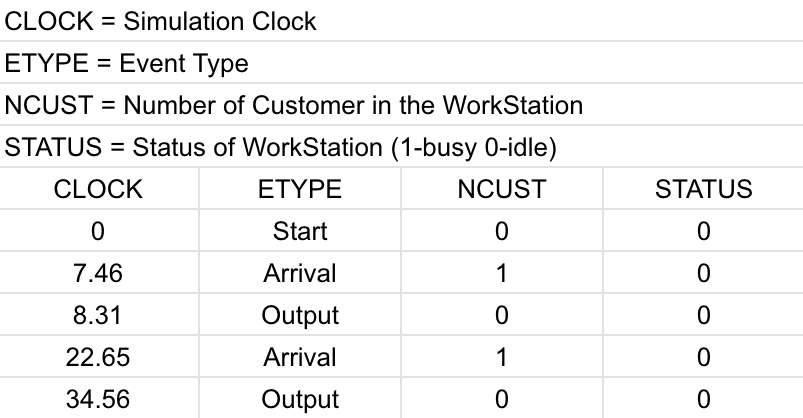
\includegraphics[width=4in]{Simulationtrace.png}
\caption{Simulation Trace}
\label{default}
\end{center}
\end{figure}

\begin{figure}[htbp]
\begin{center}
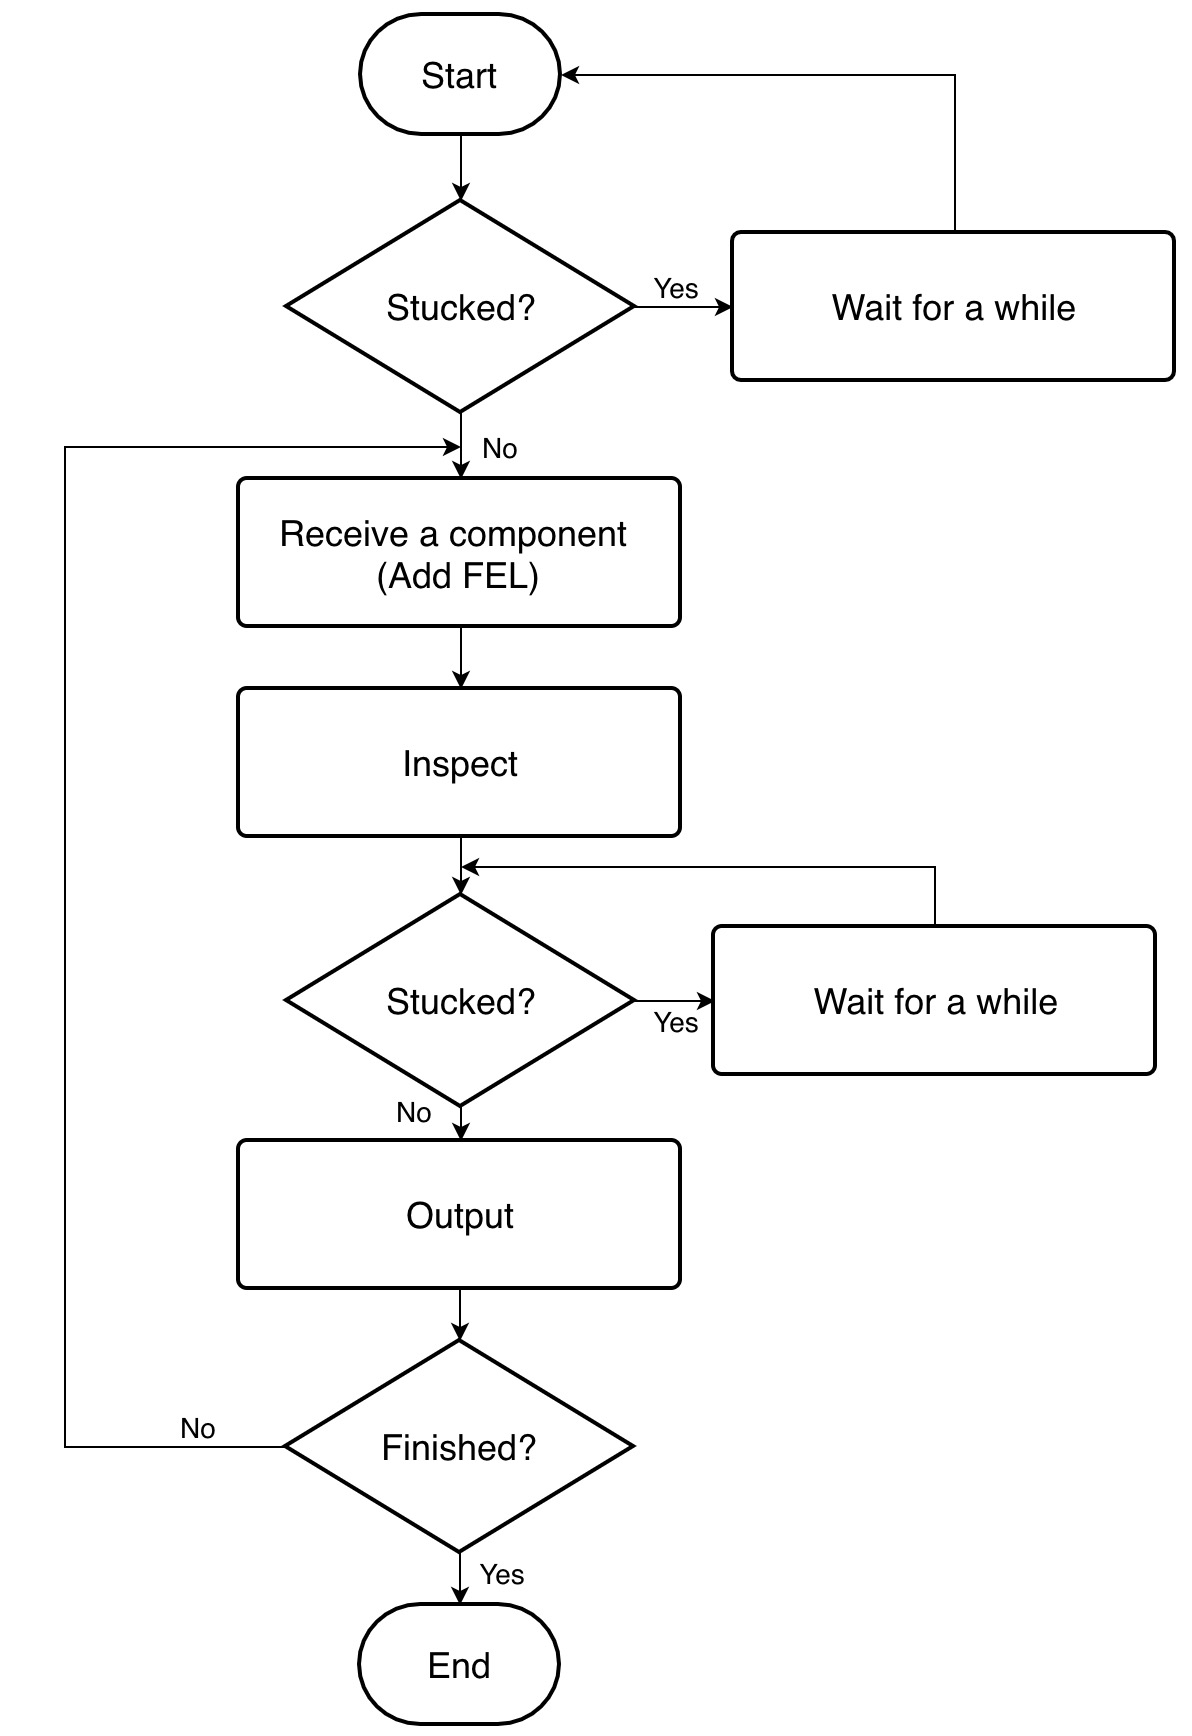
\includegraphics[width=4in]{Flowchartsp.png}
\caption{Work flow of Inspectors}
\label{default}
\end{center}
\end{figure}

\begin{figure}[htbp]
\begin{center}
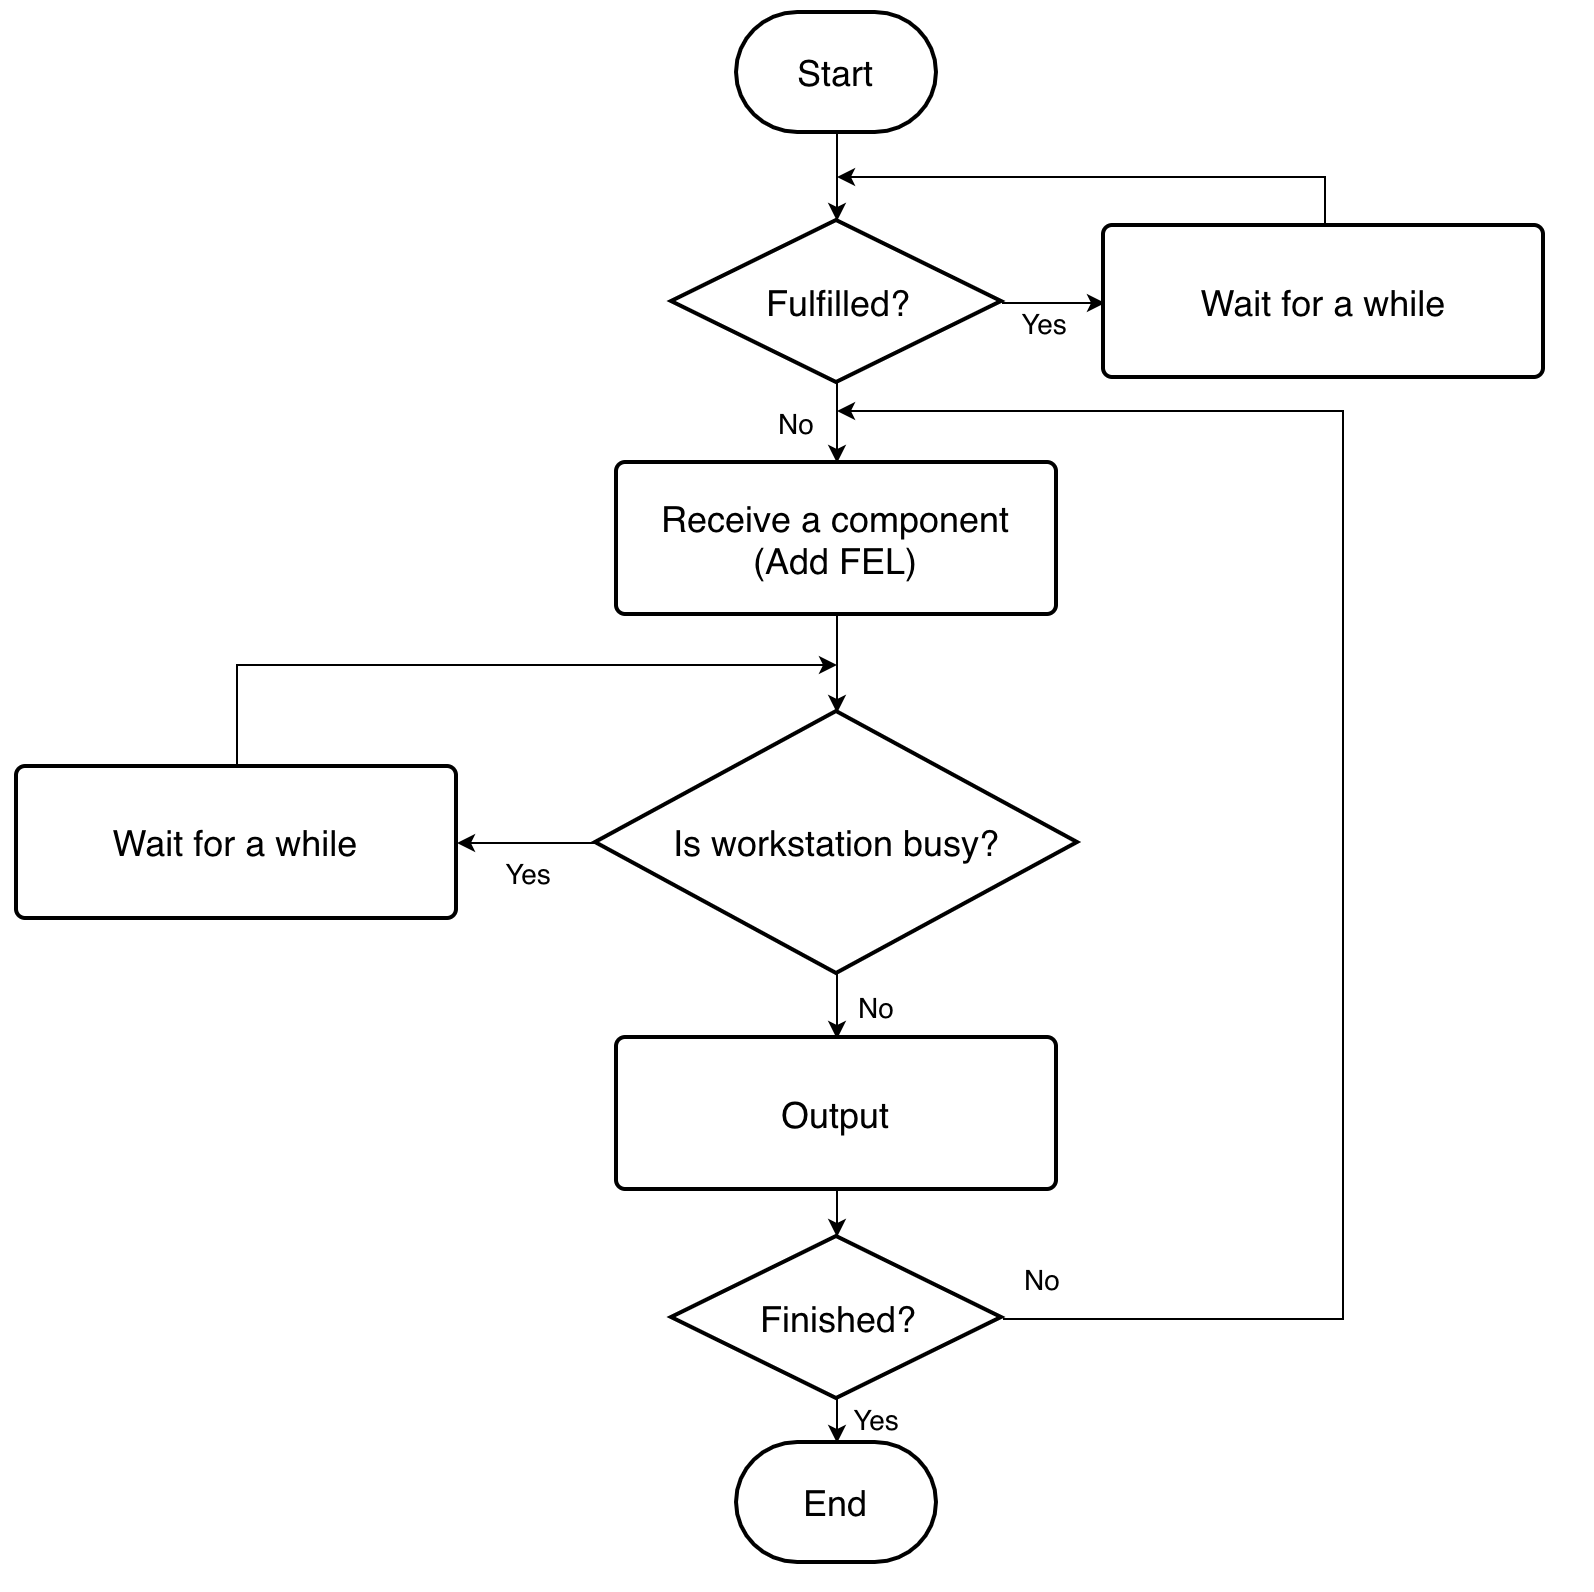
\includegraphics[width=4in]{Flowchartbuffer.png}
\caption{Work flow of Buffer}
\label{default}
\end{center}
\end{figure}

\begin{figure}[htbp]
\begin{center}
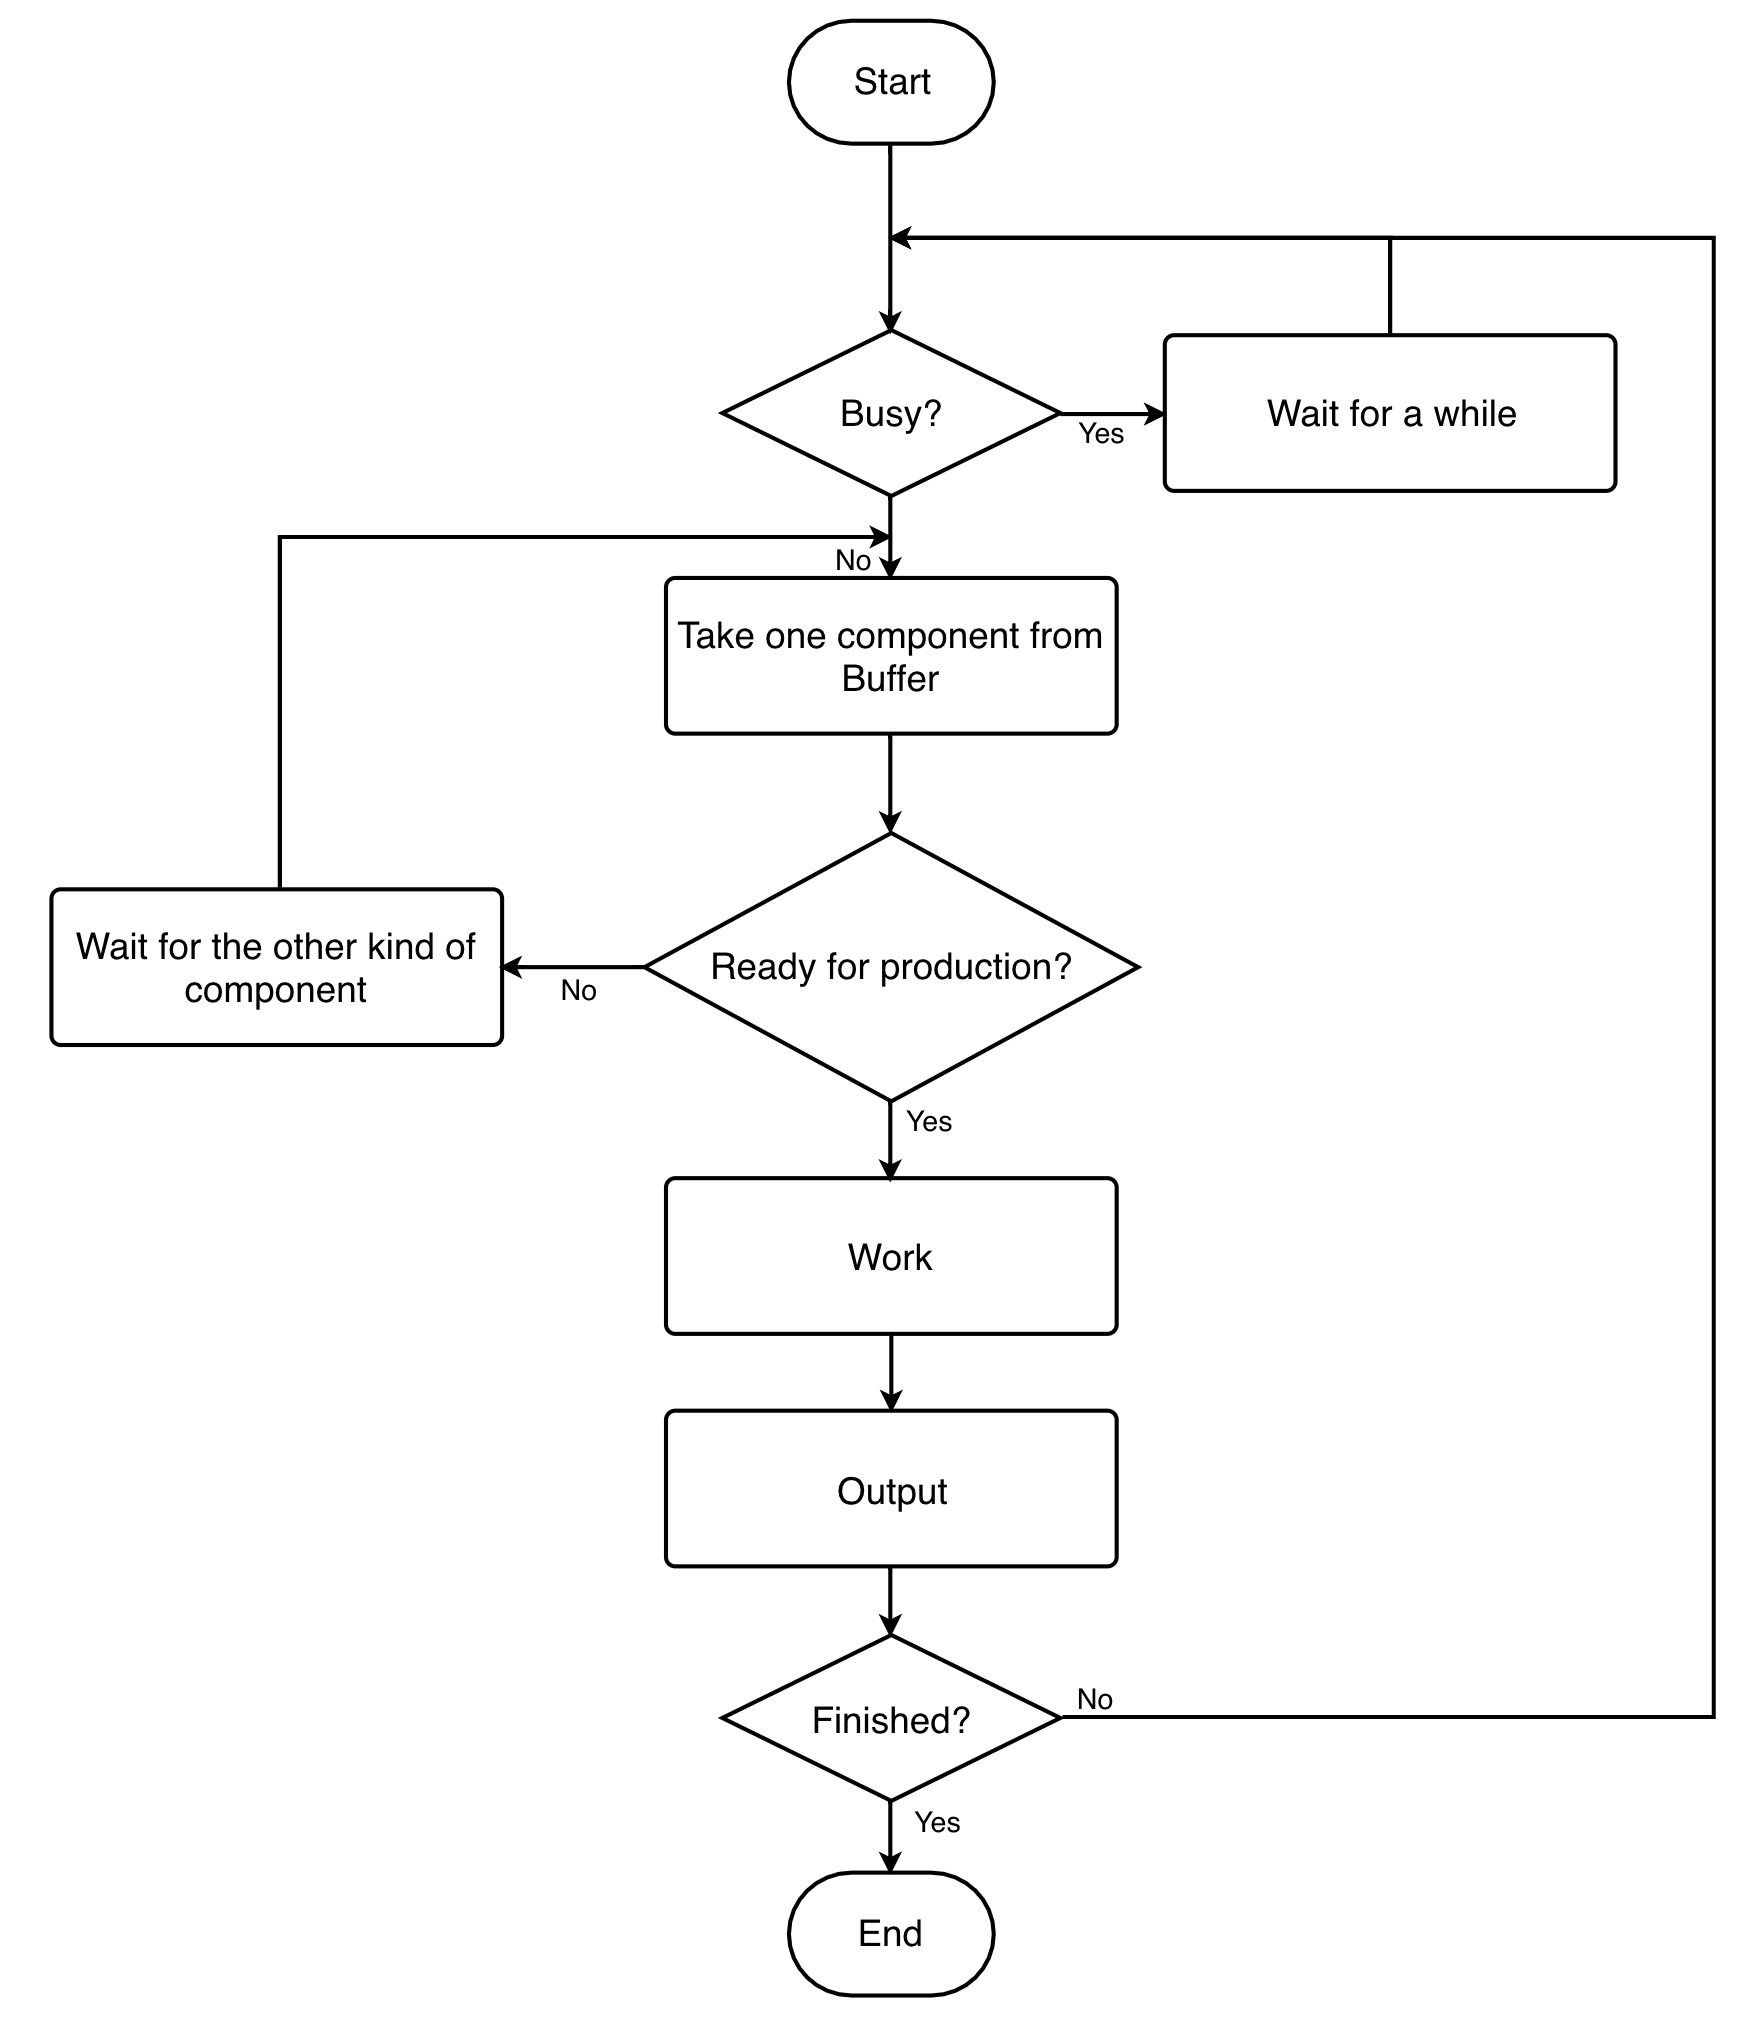
\includegraphics[width=4in]{Flowchartws.png}
\caption{Work flow of Workstation}
\label{default}
\end{center}
\end{figure}


This simulation trace table indicates how the Workstation 1 work in this process. It just wait for Component 1, deal with it and then output. If the station is busy and a new one comes, the new arrival will stay at the buffer for now.

\subsubsection{Model Output}

The output of model is reasonable because it tracks each component of the whole process and the total time it costs is similar to the real time cost. For each object in the process, I can extract what it is doing at a certain point in time.

\subsubsection{Sequence of dealing events}

My code follows the rule that proceed events as time goes. The primary key of every event happened in this process is the clock. When we know that something is certain to happen, we put it in the FEL. Then we sort it according to the time of the occurrence of these things. The earlier event comes out first and latter event comes out the last. 

\subsubsection{Little's Law}

Little's Law works for any blackbox, where the blackbox can be a complex system, or  any subunit such as a single waiting line or a single server, a waiting line plus a sever, etc. 

For each queue system in this project, we do a Little's law verification.
\begin{equation}
\hat L = \hat \lambda \hat w
\end{equation}
$\hat L$ means average number of components in the queue. $\hat \lambda$ means the arrival rate of components. $\hat w$ means average working time for each component.

For Inspector system, consider the supply of the component for each inspector is sufficient, which means theres always a component waiting outside and there's always existing one component in each inspector. It's easy to calculate that the average dealing time for each inspector but things are little different here. If the corresponding workstation has a full buffer already and can't hold more components, the component must stay in the inspector and the inspector stop receiving new components. Here we have $L=\hat L =1, \hat w = 10.36, \hat \lambda = 0.10$. It follows Little's law. By checking to see if these averages are in range, we can verify quickly if the system is wrong before we even look at any other part of the simulation.
Here we have the number of each component in each buffer of the specific workstation.

\begin{figure}[htbp]
\begin{center}
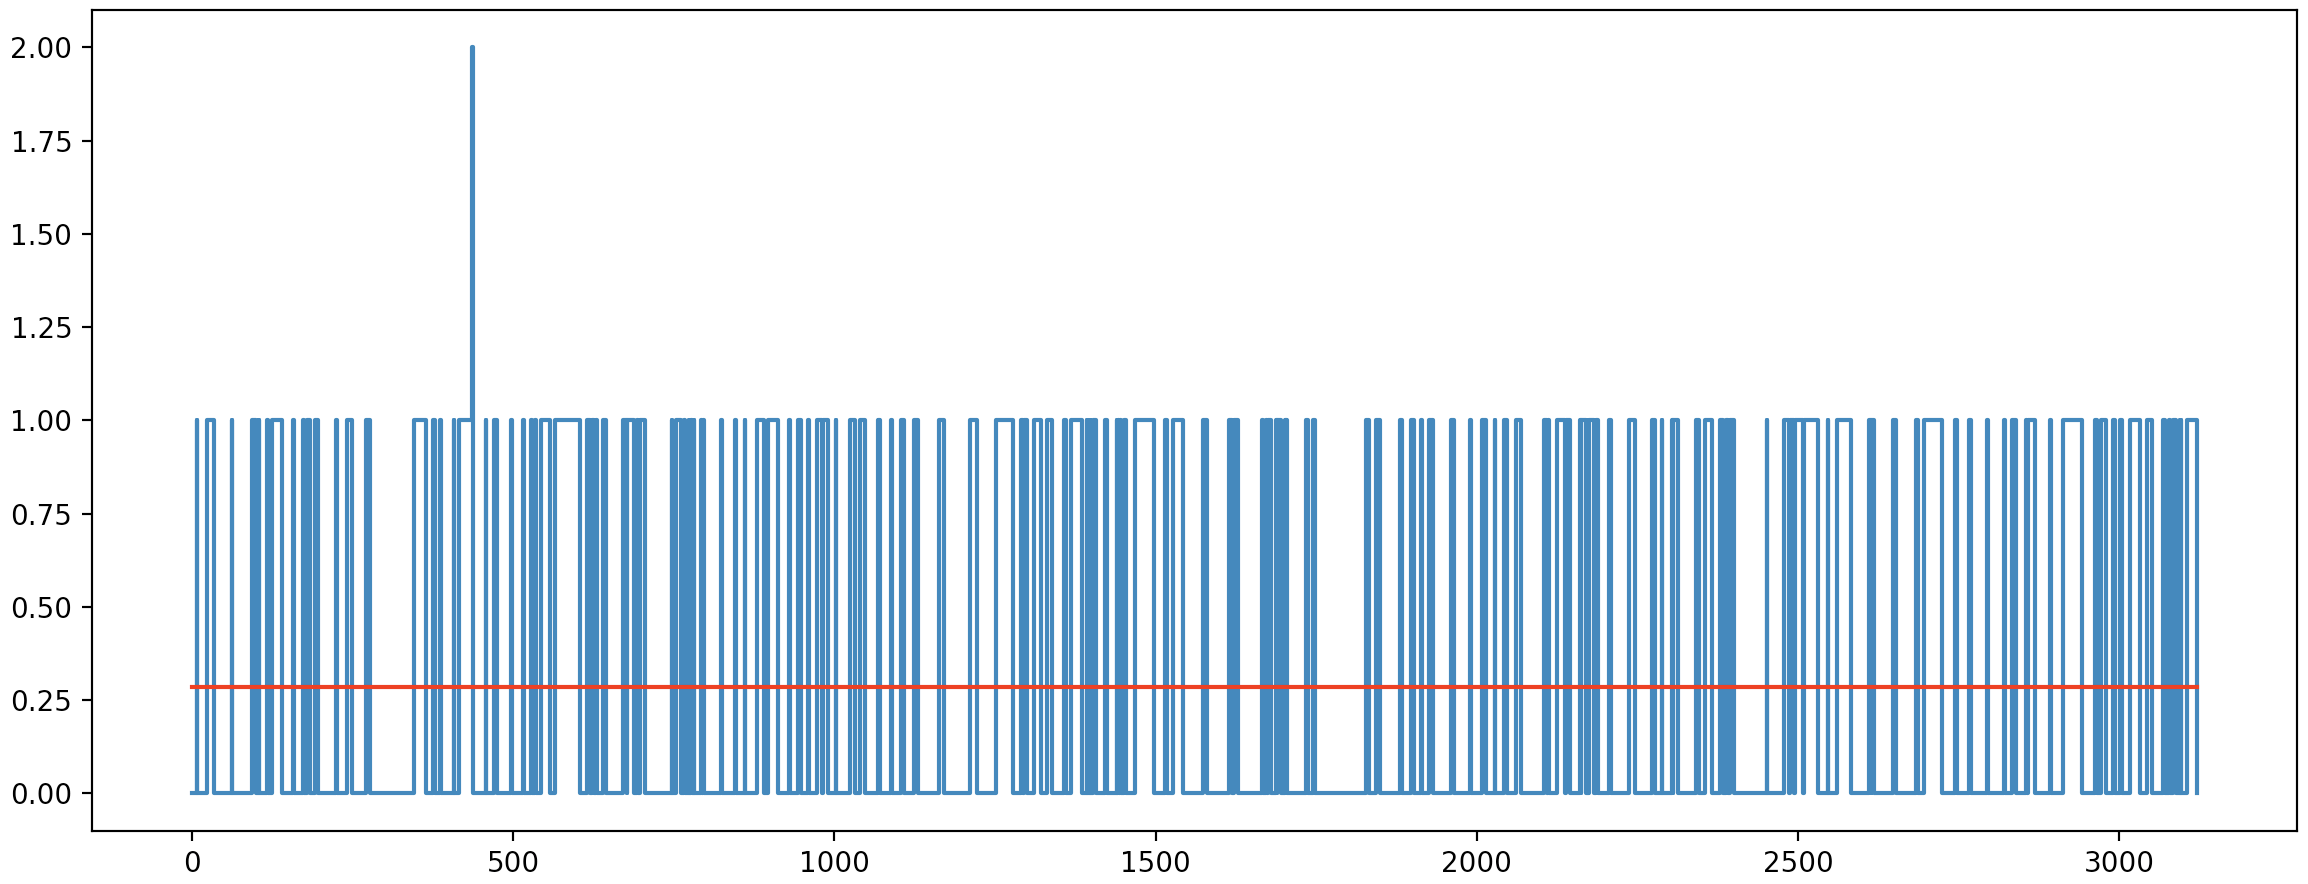
\includegraphics[width=4in]{W1_C1B.png}
\caption{The number of components in Component 1 buffer of Workstation 1}
\label{W1_C1B}
\end{center}
\end{figure}

The x axle on the diagram shows the time line of the whole process of production, while the y axle indicates how many kind of this components in the buffer at this time. I also draw a red mean line to denote the average number of gears in buffer in this period. 

Verification: $L = 0.286, \lambda = 0.06, w = 5.19$

\begin{figure}[htbp]
\begin{center}
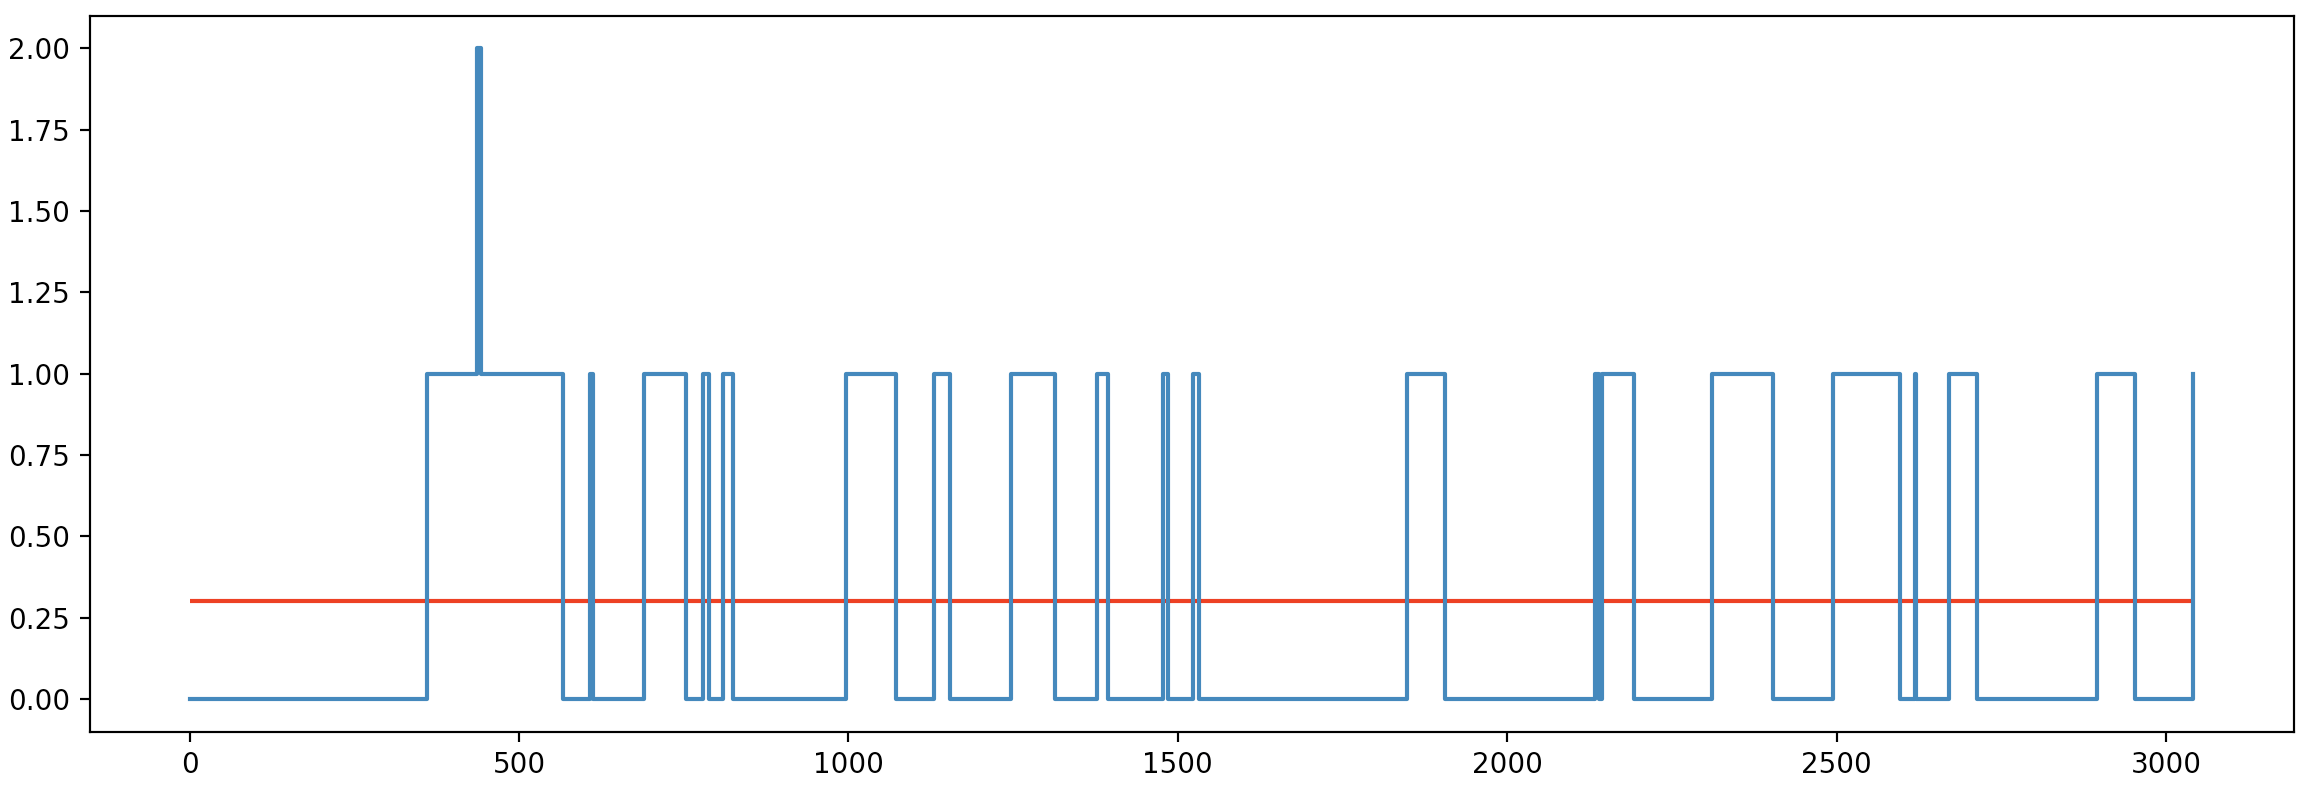
\includegraphics[width=4in]{W2_C1B.png}
\caption{The number of components in Component 1 buffer of Workstation 2}
\label{W2_C1B}
\end{center}
\end{figure}

\begin{figure}[htbp]
\begin{center}
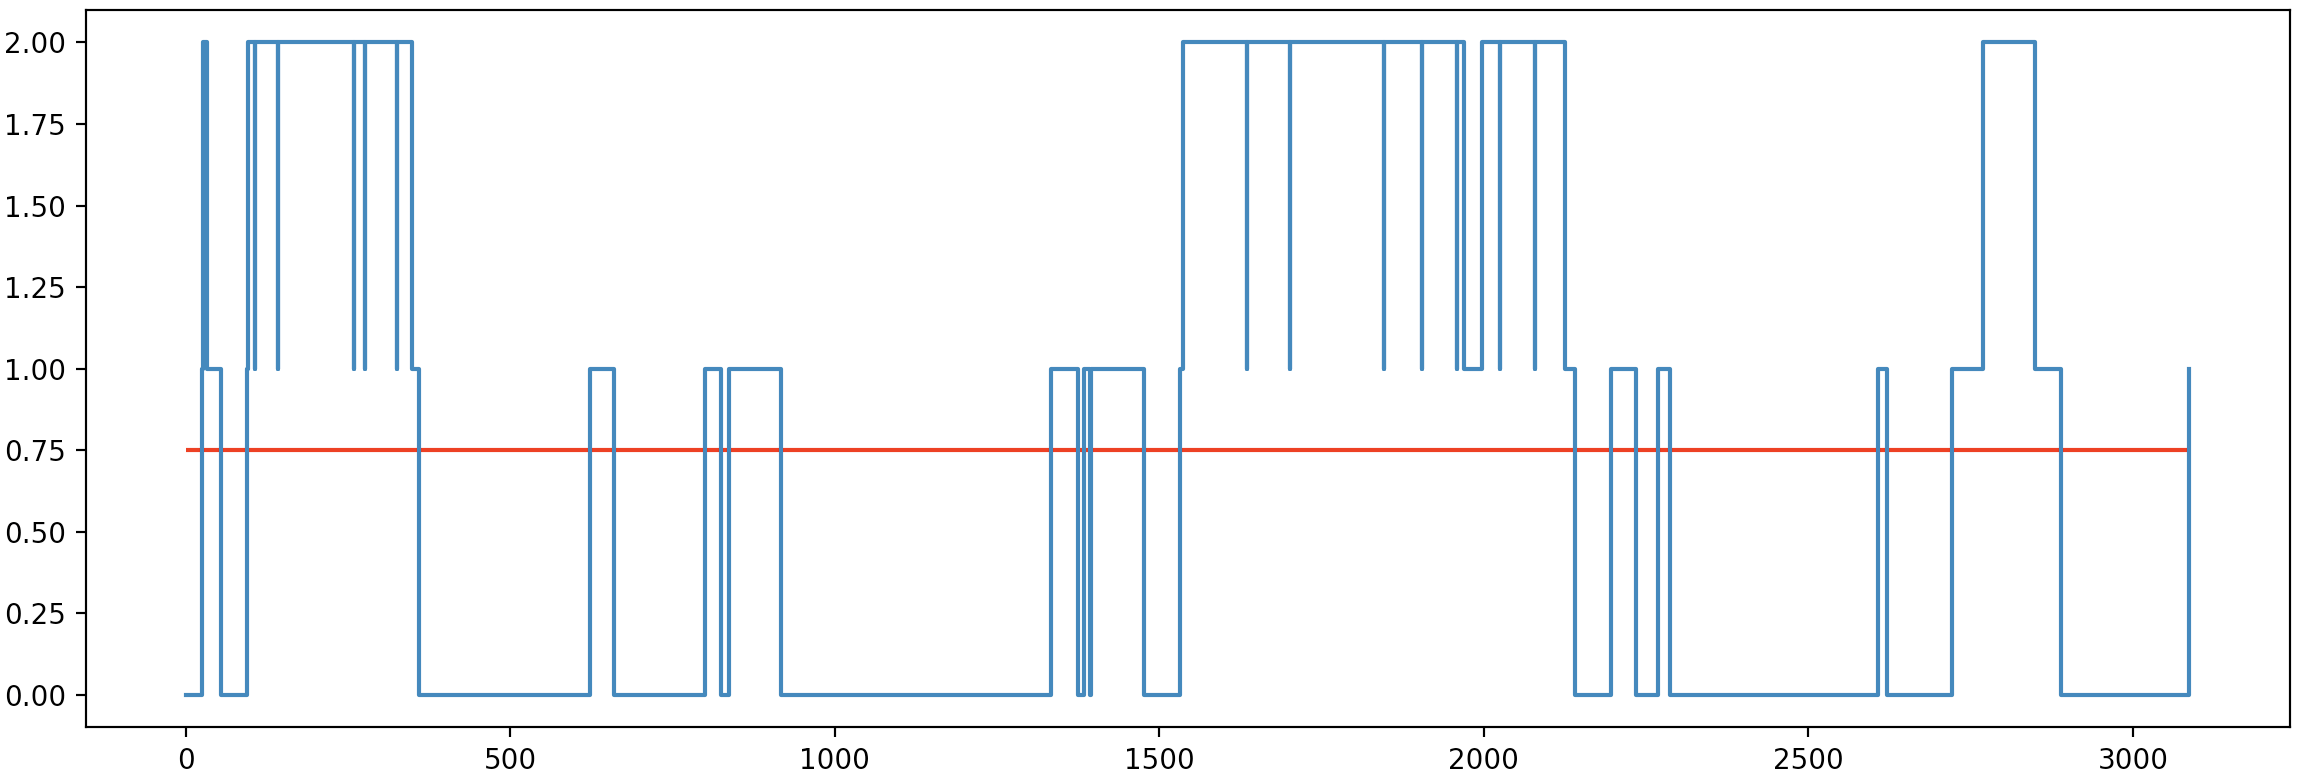
\includegraphics[width=4in]{W2_C2B.png}
\caption{The number of components in Component 2 buffer of Workstation 2}
\label{W2_C2B}
\end{center}
\end{figure}

\begin{figure}[htbp]
\begin{center}
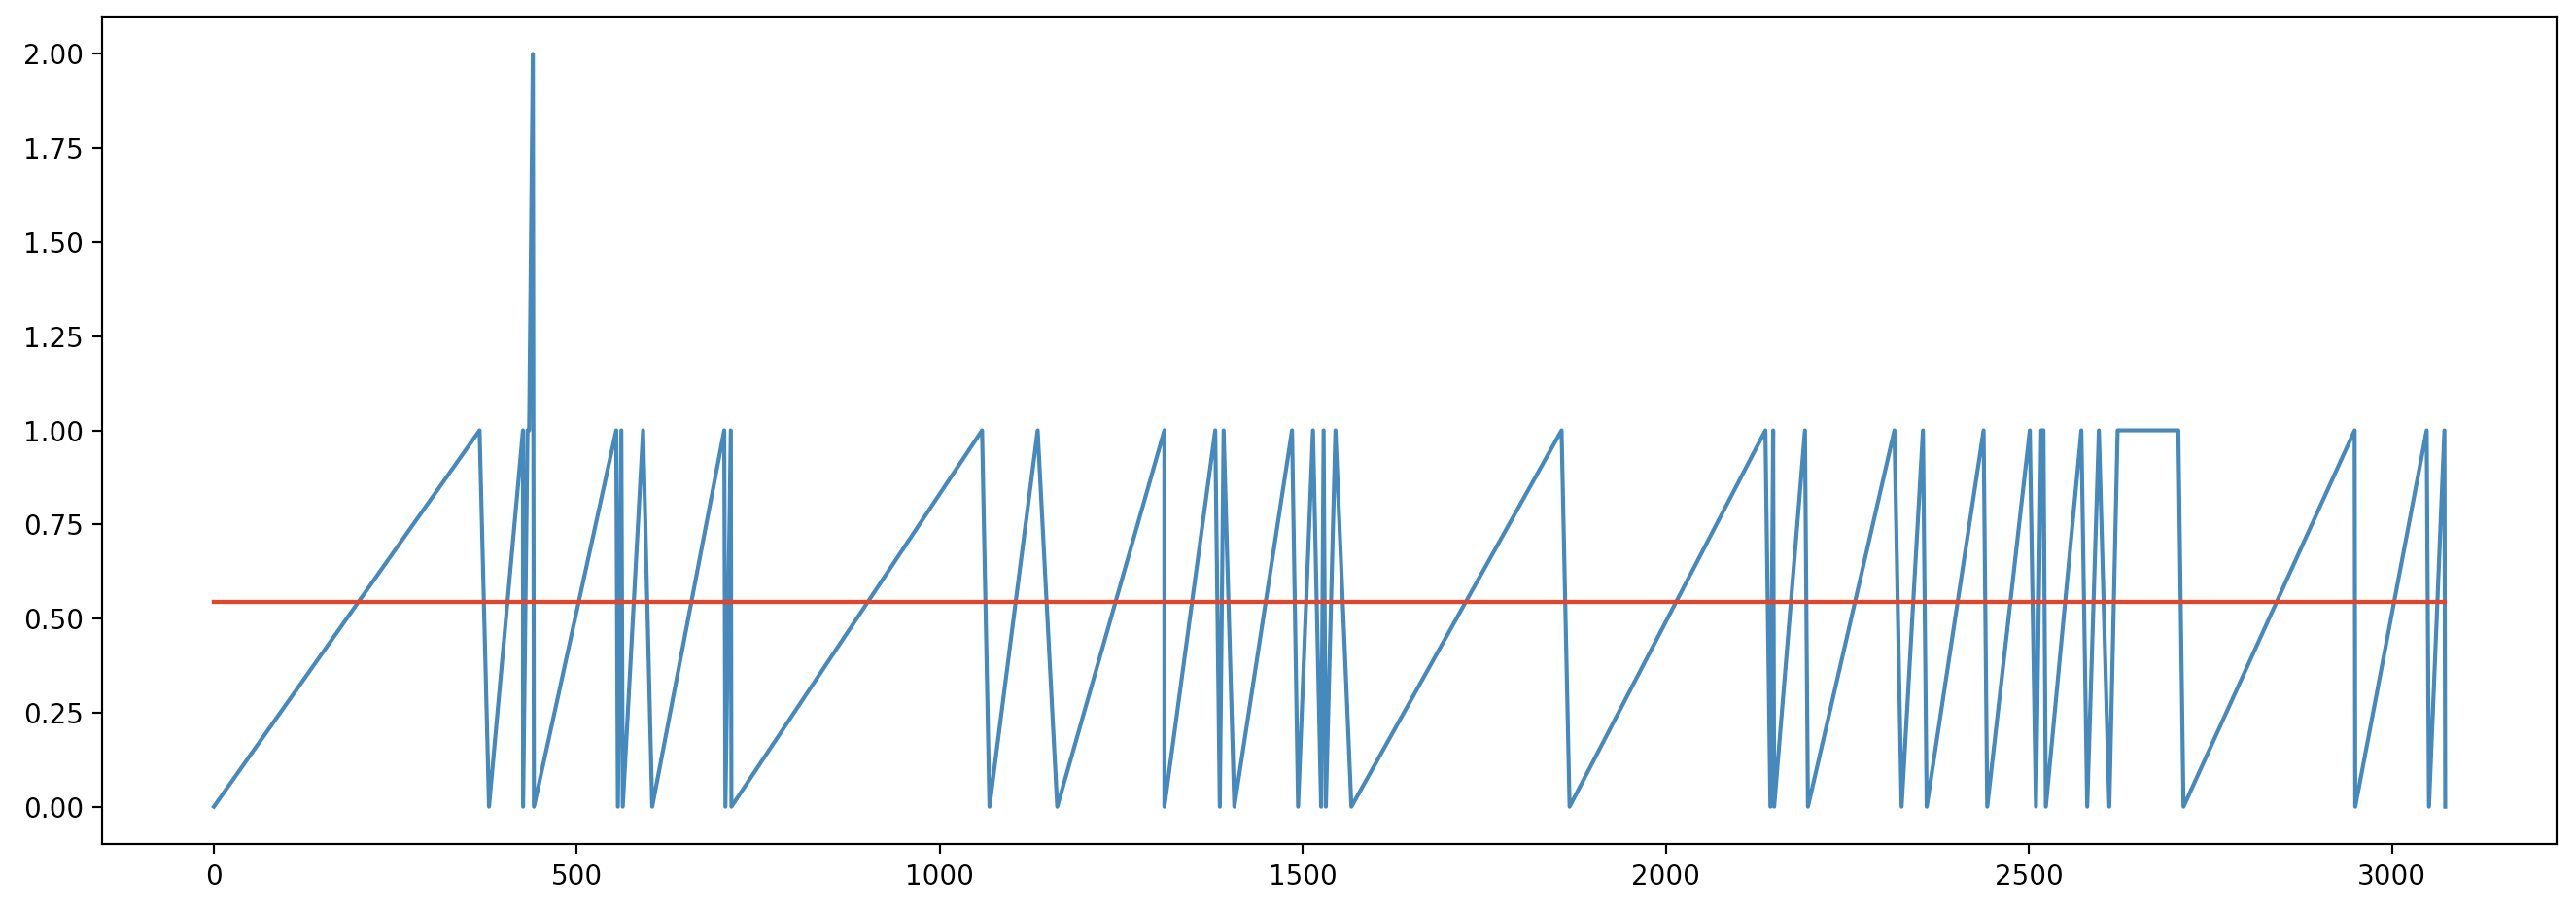
\includegraphics[width=4in]{W3_C1B.png}
\caption{The number of components in Component 1 buffer of Workstation 3}
\label{W3_C1B}
\end{center}
\end{figure}

\begin{figure}[htbp]
\begin{center}
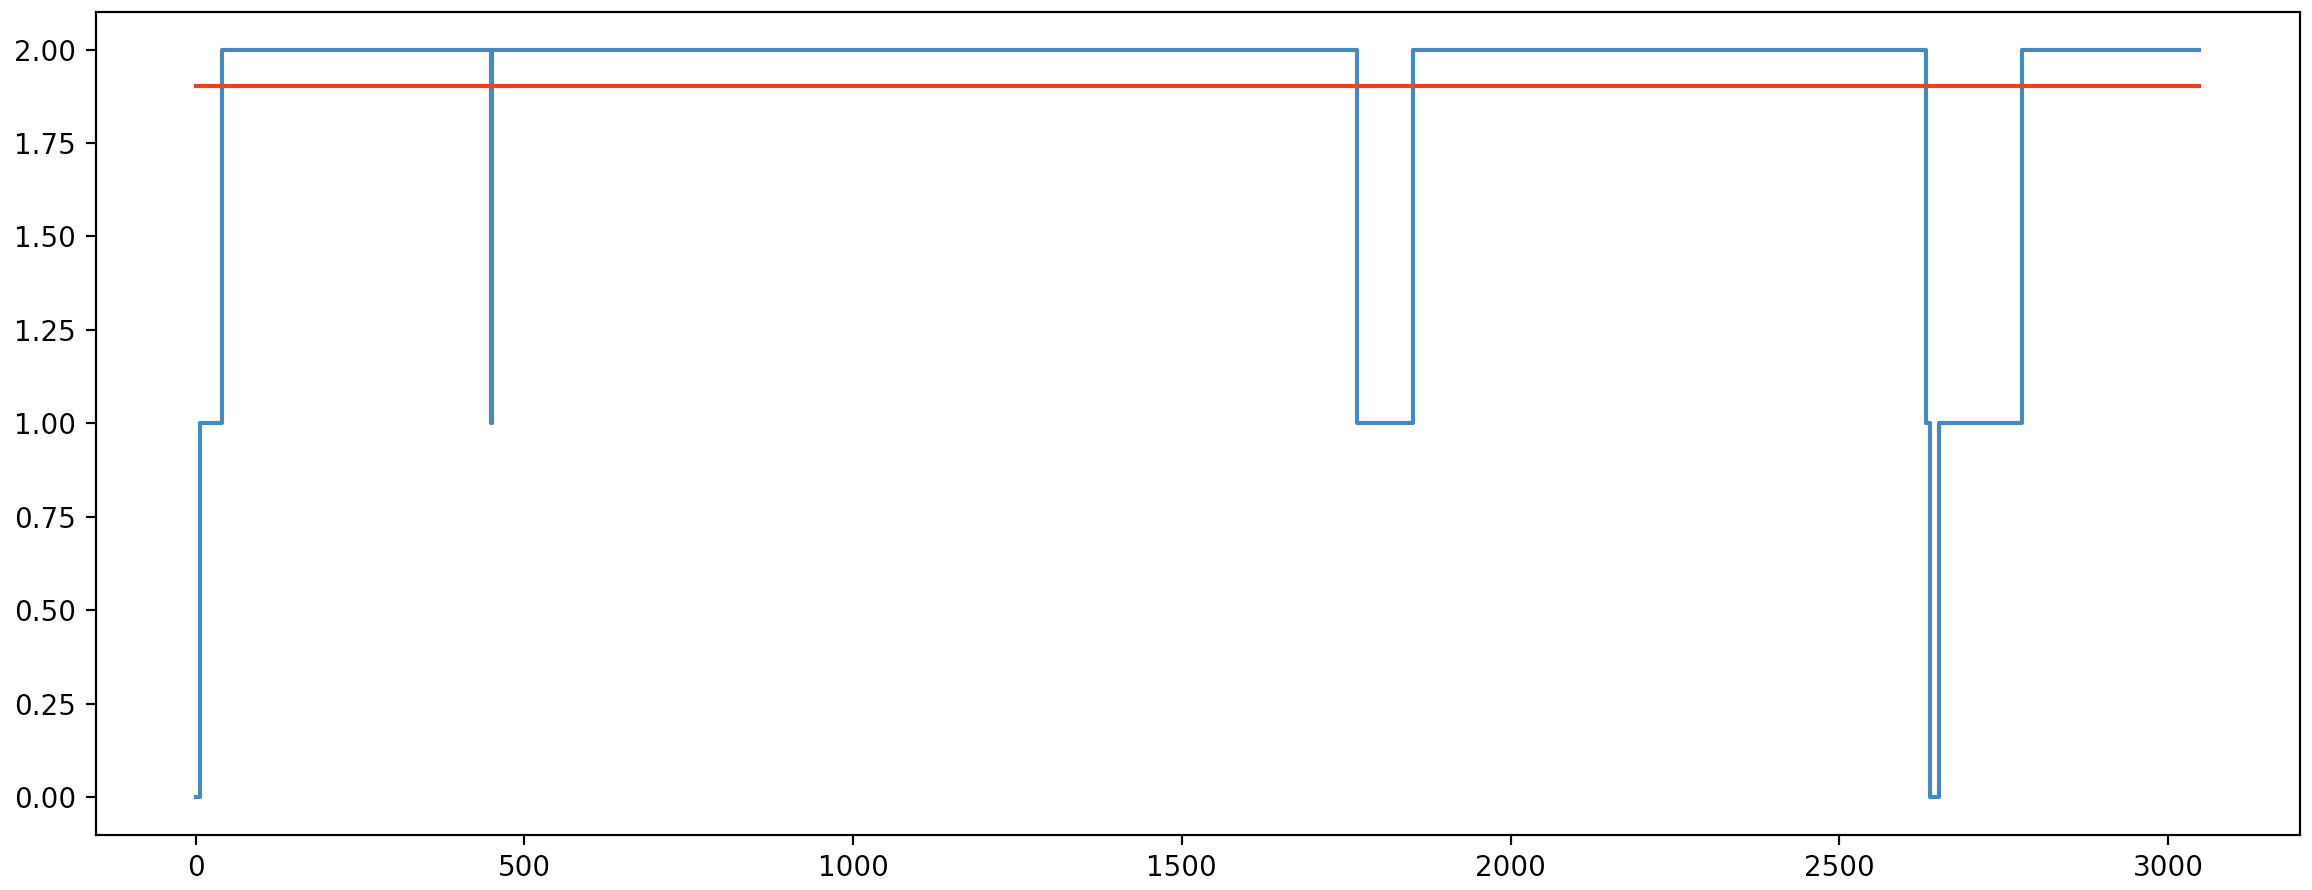
\includegraphics[width=4in]{W3_C3B.png}
\caption{The number of components in Component 3 buffer of Workstation 3}
\label{W3_C3B}
\end{center}
\end{figure}


\subsection{Validation}

\subsection{Face Validity}






\end{document}